\documentclass[12pt,a4paper]{report}
\usepackage[utf8]{inputenc}
\usepackage[portuguese]{babel}
\usepackage{titlesec}
\usepackage{graphicx}
\usepackage{indentfirst}
\usepackage{enumerate}
\usepackage{float}
\usepackage{array}
\usepackage{tikz}
\usepackage{multirow}
\usepackage{multicol}
\usepackage{geometry}
\usepackage[cache=false]{minted}
\usepackage{pdflscape}
\usepackage[titletoc]{appendix}
\usepackage{hyperref}
\geometry{
 a4paper,
 top=2cm,
 bottom=2cm,
 left=3cm,
 right=3cm
}
\addto\captionsportuguese{
      \renewcommand{\contentsname}
          {Índice}
}
\titleformat{\chapter}{\normalfont\huge}{\thechapter.}{30pt}{\bf\huge}
\begin{document}

\newcommand{\outputStart}[0]{$>>>$}
\newcommand{\outputEnd}[0]{$<<<$}

\begin{titlepage}
    \center
    {\huge {\bf Universidade do Minho}}\\[0.4cm]
    \vspace{3.0cm}
    \textsc{\huge{Processamento de notebooks}}\\[0.5cm]
    \vspace{3.0cm}
    \textsc{\huge{Mestrado Integrado em Engenharia Informática}}\\[0.5cm]
    \vspace{2.0cm}
    \textsc{Sistemas Operativos}\\[0.5cm]
    \textsc{(2º Ano, 2º Semestre, 2017/2018)}\\[0.5cm]
    \vspace{1.5cm}
    \begin{flushleft}
        A79003 \,\,\,Pedro Mendes Félix da Costa
        \vspace{0.2cm}

        A80453 \,\,\,Bárbara Andreia Cardoso Ferreira
        \vspace{0.2cm}

        A82145 \,\,\,Filipa Parente
    \end{flushleft}
        \vspace{1cm}
    \begin{flushright}
        Braga

        Maio 2018
    \end{flushright}

\end{titlepage}

\tableofcontents
\clearpage

\chapter{Introdução}
    Este trabalho foi realizado no âmbito da unidade curricular sistemas
    operativos e tem como objetivo o processamento de ficheiros de texto
    com comandos de bash alterando estes para incluir o \textit{output} destes.

    Este processamento foi implementando com recurso a \textit{system calls}
    e à criação de multiplos processos para que houvesse o maximo de
    paralelismo possivel.

\chapter{Descrição do Problema}
    Os ficheiros de texto a ser processados, chamados \textit{notebooks}, podem
    conter 3 tipos de conteudo:
    \begin{itemize}
        \item Comentarios
        \item Commandos
        \item Output
    \end{itemize}
    \section{Comentarios}
        Texto simples que não é alterado de forma alguma durante o
        processamento. Estes não podem começar por \$, '\outputStart' ou
        '\outputEnd'.
    \section{Comando}
        Linha começada por \$ que contem o comando que vai ser executado.
        Este tipo de linha suporta multiplas opções adicionais.
        \subsection{Pipe para um comando anterior}
            Se, seguido do \$, estiver um número N e um $|$ o input do commando
            será obtido do commando que estiver N posições acima no ficheiro.
            Caso este número seja 1 este pode ser omitido.
        \subsection{Pipelining numa so linha}
            Um commando pode ser na verdade um encadeamento de varios comandos
            unidos por pipes, por exemplo
            \mintinline{bash}{grep -v ˆ# /etc/passwd | cut -f7 -d: | uniq},
            neste caso o comportamento é o esperado: O input desta sequência
            poderá ser obtido de um commando anterior e o seu output
            redirecionado para um proximo commando no ficheiro.
        \subsection{Execução em paralelo}
            Num so linha começada por \$ varios commandos podem ser executados
            separados por \&. Neste caso os seu output é misturado,
            indiscrimidamente na sua secção de output. Caso esta linha esteja
            a receber input de uma anterior, este input é distribuido para
            todos os commandos separados por \&. Inversamente, caso algum
            commando esteja a receber o seu input desta linha, este receberá
            o output de todos os comandos presentes nesta linha também por
            ordem "aleatoria".
        \subsection{Redirecionamento para ficheiros}
            Uma linha de comando suporta também o Redirecionamento para
            ficheiros usando a sintaxe usual da \textit{bash}:
            \mintinline{bash}{<, >, >>, 2>, &>}.
            Quando este tipo de redirecionado é utilizado, no entanto,
            impossibilita algumas das opções anteriores, por exemplo,
            se o output for redirecionado para um ficheiro, nenhum dos commandos
            seguintes pode depender deste output.

\chapter{Parsing}
    Para fazer o \textit{parsing} do notebook foi concebida uma estrutura
    dinamica que vai verificando se o ficheiro está construido corretamente
    enquanto organiza o seu conteudo de forma a, posteriormente, poder ser
    processado mais facilmente.

    A estrutura em sí é um array dinamico de \textbf{Node}s que podem ser
    commentários ou comandos. Caso seja um comentário trata-se apenas de
    uma string.
    \begin{figure}[h]
        \centering
        \begin{minted}{C}
            struct _comment{
                String comment;
            };
        \end{minted}
        \caption{Representação em memória de um comentário}
        \label{fig:commentStruct}
    \end{figure}

    Caso seja um comando é guardada bastante informação sobre este.
    \begin{figure}[h]
        \centering
        \begin{minted}{C}
            struct _command{
                size_t dependency;
                String command;
                String output;
                IdxList dependants;
                Command pipe;
            };
        \end{minted}
        \caption{Representação em memória de um comando}
    \end{figure}

    A função de cada um dos campos é, respetivamente:
    \begin{itemize}
        \item \mintinline{C}{dependency}: Quantas posições atráz está o commando
            de, cujo output, este depende. Se este número for 0 o commando não
            depende.

        \item \mintinline{C}{command}: O commando em sí. Neste ponto não são
            incluidos o \$ nem o $|$ e/ou números presentes no inicio da linha
            do notebook.

        \item \mintinline{C}{output}: O output deste commando. Inicialmente
            começa vazio e tem de ser mais tarde preenchido.

        \item \mintinline{C}{dependants}: O array das posições onde estão os
            comandos que dependem do output deste.

        \item \mintinline{C}{pipe}: O apontador para o proximo comando na
            \textbf{Batch}.
    \end{itemize}

    \section{Batches}
        A organização dos comandos é feita sobre a forma de batches. Os comandos
        que estejam interligados de alguma forma estão todos colocados na mesma
        lista ligada, designada batch. Desta forma é possivel definir blocos do
        notebook que são independentes uns dos outros para que possam ser
        executados de forma paralela.

    \section{Ilustração da estrutura}
        Dada esta organização um exemplo de como um notebook é traduzido para
        esta estrutura pode ser o seguinte:

        \begin{figure}[H]
            \begin{minted}{text}
                            Comentario 1
                            $ ls
                            $| grep .c
                            Comentário 2
                            $ ps
                            $| wc
                            $2| head -2
                            $5| tail -2
            \end{minted}
            \caption{Notebook exemplo com dois batches}
        \end{figure}
        \begin{figure}[H]
            \centering
            \usetikzlibrary{matrix,backgrounds,positioning,calc,fit}
\definecolor{commentColor}{RGB}{102,102,102}
\definecolor{commandColor}{RGB}{59,61,196}

\begin{tikzpicture}[font=\ttfamily,
varray/.style={
    matrix of nodes,nodes={
        draw, minimum size=10mm, fill=white!30},
    column sep=-\pgflinewidth,
    row sep=-\pgflinewidth,
    nodes in empty cells,
    column 1/.style={
        nodes={
            draw=none, fill=none, minimum size=5mm
        }
    }
},
harray/.style={
    matrix of nodes, nodes={
        draw, minimum size=2mm, fill=white!30},
    column sep=-\pgflinewidth,
    row sep=-\pgflinewidth,
    nodes in empty cells,
    row 1/.style={
        nodes={
            draw=none, fill=none, minimum size=5mm
        }
    }
},
cmdPtr/.style={
    draw, commandColor, fill=commandColor, minimum size=2mm, circle
},
cmtPtr/.style={
    draw, commentColor, fill=commentColor, minimum size=2mm, circle
}]

\newdimen\zerolinewidth

\tikzset{
    zero line width/.code={
        \zerolinewidth=\pgflinewidth
        \tikzset{line width=0cm}
    },
    use line width/.code={
        \tikzset{line width=\the\zerolinewidth}
    },
    anchor-in-boundary/.style={
        zero line width,
        postaction={draw,use line width},
    },
}

\matrix[varray] (parseTree) {
0 &    \\
1 &    \\
2 &    \\
3 &    \\
4 &    \\
5 &    \\
6 &    \\
};
\draw (parseTree-1-2.north)++ (60:0mm) node [above] (ptLabel) {Parse Tree};

% Comment 1
    \node[cmtPtr] at (parseTree-1-2) (cmt1ptr) {};
    \node[draw, commentColor, right = 20pt of parseTree-1-2.east]
        (cmt1) {'Comentario 1'};
    \draw[->, thick] (cmt1ptr)--(cmt1);

% Command 1 LS
    \node[cmdPtr] at (parseTree-2-2) (cmdLSPtr) {};
    \node[draw, commandColor, text=black, right = 20pt of parseTree-2-2.east]
        (cmdLS) {ls};
    \draw (parseTree-2-1.west)++(0:0mm) node [left, text=red]
        (batch0Label) {Batch 0};

% Command 2 Grep
    \node[cmdPtr] at (parseTree-3-2) (cmdGrepPtr) {};
    \node[draw, commandColor, text=black, right = 20pt of cmdLS.east]
        (cmdGrep) {grep .c};

% Comment 1
    \node[cmtPtr] at (parseTree-4-2) (cmt2ptr) {};
    \node[draw, commentColor, right = 20pt of parseTree-4-2.east]
        (cmt2) {'Commentario 2'};
    \draw[->, thick] (cmt2ptr)--(cmt2);

% Command 3 PS
    \node[cmdPtr] at (parseTree-5-2) (cmdPSPtr) {};
    \node[draw, commandColor, text=black, right = 20pt of parseTree-5-2.east]
        (cmdPS) {ps};
    \draw (parseTree-5-1.west)++(0:0mm) node [left, text=red]
        (batch1Label) {Batch 1};

% Command 4 Head
    \node[cmdPtr] at (parseTree-6-2) (cmdHeadPtr) {};
    \node[draw, commandColor, text=black, right = 20pt of cmdPS.east]
        (cmdHead) {head -2};

% Command 5 Tail
    \node[cmdPtr] at (parseTree-7-2) (cmdTailPtr) {};
    \node[draw, commandColor, text=black, right = 20pt of cmdGrep.east]
        (cmdTail) {tail -2};

\foreach \from/\to in {cmdLSPtr/cmdLS, cmdLS/cmdGrep, cmdGrep/cmdTail,
                        cmdPSPtr/cmdPS, cmdPS/cmdHead}
    \draw [->, thick] (\from)--(\to);

\draw[->, thick, bend right=18] (cmdGrepPtr) edge (cmdGrep);

\draw[->, thick, bend right=18] (cmdHeadPtr) edge (cmdHead);

\draw[->, thick, bend right=45] (cmdTailPtr) edge (cmdTail);

\end{tikzpicture}

            \caption{Representação em memória do notebook}
        \end{figure}

        Neste exemplo podemos ver que foram produzidos 2 batches. O Batch 0 é
        constituido pelo \mintinline{bash}{ls}, \mintinline{bash}{grep .c} e
        \mintinline{bash}{tail -2}. O Batch 1 é constituido pelo
        \mintinline{bash}{ps} e pelo \mintinline{bash}{head -2}.

\chapter{Execução de commandos}

    \section{Processo Pai}
        Feito o parsing, da-se inicio à execução dos commandos. Primeiro o
        processo pai cria um filho para cada batch e, de seguida, espera que
        estes morram para receber os resultado acumulado dos commandos
        executados por cada um atravez de um pipe. A partir deste resultado
        atualiza o output dos commandos e por fim converte a estrutura em
        texto que escreve no ficheiro.

    \section{Processo Batch}
        Cada filho ira trabalhar sobre um, batch (lista ligada de commandos),
        criando um filho para cada nó da lista. Aqui é também decidido o metodo
        de execução de cada nodo.
        \subsection{Commando simples}
            Caso seja um comando simples é apenas redirecionado o seu input e
            output para pipes que comunicam com o processo encarregue do batch a
            que pertence. Está aqui incluido também o redirecionamento para
            ficheiros, caso seja necessário.
        \subsection{Commando com pipelines}
            Caso seja um commando com pipelines o input e output é redirecionado
            de forma analoga ao caso anterior e o encadeamento é feito
            corretamente.
        \subsection{Dois ou mais commandos em paralelo}
            Caso o nodo contenha um ou mais commandos separados por \& o
            tratamento é mais complexo. Primeiro, este filho cria um outro
            filho para cada comando que o irá executar com \textit{stdin}
            e \textit{stdout} redirecionados para um pipe cada. Enquanto os
            commandos executam o pai destes, filho do batch, escreve para todos
            o input que esta a receber do seu pai (batch) e agrega todo o
            output que lê dos seus filhos e envia-o, também, para o seu pai.

\chapter{Opções de execução}
    O comportamento do programa pode ser alterado fazendo uso de \textit{flags}
    que podem ser passadas como argumento do programa.
    \section{\textit{help}}
        A flag \mintinline{text}{-h} apresenta a lista de opções possiveis
        de passar e termina execução.
    \section{Escrever para o \textit{stdout}}
        A flag \mintinline{text}{-o} faz com que o output produzido seja
        impresso para o \textit{standard output} invez de alterar o ficheiro
        de origem.
    \section{Execução sequencial}
        A flag \mintinline{text}{-s} faz com que as batches sejam executadas
        sequencialmente, ou seja, a batch n só é executada quando a batch n-1
        terminar.
    \section{Ler do \textit{stdin}}
        Se o nome do ficheiro for \mintinline{text}{-} o input do programa será
        obtido do \textit{standard input} invez de obtido de um ficheiro. Esta
        opção automaticamente ativa a opção de escrever para o \textit{stdout}.

\chapter{Controlo de erros}
    Durante a fase de \textit{parsing} são detetados erros de sintaxe que possam
    existir, caso algum seja detetado o processamente é abortado e uma mensagem
    a indicar o erro que ocurreu é impressa para o \textit{stderr}.

    \begin{figure}[h]
        \centering
        %\captionsetup{width=0.5\textwidth}
        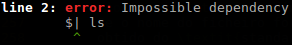
\includegraphics[width=0.5\textwidth]{./images/parseError.png}
        \caption{Messagem de erro enviada caso seja pedida uma dependencia
                    impossivel}
        \label{fig:parseError}
    \end{figure}

    Durante a execução dos commandos se algum destes fizer o
    \mintinline{C}{execvp()} falhar a execução de todos os outros é interrompida
    e o ficheiro fonte permanece inalterado.

    \begin{figure}[h]
        \centering
        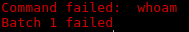
\includegraphics[width=0.5\textwidth]{./images/execError.png}
        \caption{Erro apresentado no ecra caso o commando não exita. Neste caso
                    para o comando \mintinline{text}{whoam}}
    \end{figure}

\chapter{Conclusões e Trabalho Futuro}
    Em suma, o grupo considera que o trabalho foi realizado na sua
    totalidade de forma estruturada, respondendo a todos os requisitos e ainda
    adicionando requisitos não pedidos explicitamente.

    Um aspeto que poderia ser melhorado era permitir que o output fosse
    redirecionado de e para ficheiros sem comprometer as restantes
    funcionalidades, no entanto, esta falha pode ser contornada com as opções
    implementadas, apesar de ser menos eficiente.

\end{document}
